%!TEX TS-program = xelatex
%!TEX options = -aux-directory=Debug -shell-escape -file-line-error -interaction=nonstopmode -halt-on-error -synctex=1 "%DOC%"
\documentclass{article}
\input{LaTeX-Submodule/template.tex}

% Additional packages & macros
\usepackage{mathdots}

\DeclareMathOperator*{\argmax}{arg\,max}
\DeclareMathOperator*{\argmin}{arg\,min}
\DeclareMathOperator*{\nullity}{nullity}

% Header and footer
\newcommand{\unitName}{Advanced Linear Algebra}
\newcommand{\unitTime}{Semester 1, 2022}
\newcommand{\unitCoordinator}{Prof Timothy Moroney}
\newcommand{\documentAuthors}{\textsc{Tarang Janawalkar}}

\fancyhead[L]{\unitName}
\fancyhead[R]{\leftmark}
\fancyfoot[C]{\thepage}

% Copyright
\usepackage[
    type={CC},
    modifier={by-nc-sa},
    version={4.0},
    imagewidth={5em},
    hyphenation={raggedright}
]{doclicense}

\date{}

\begin{document}
%
\begin{titlepage}
    \vspace*{\fill}
    \begin{center}
        \LARGE{\textbf{\unitName}} \\[0.1in]
        \normalsize{\unitTime} \\[0.2in]
        \normalsize\textit{\unitCoordinator} \\[0.2in]
        \documentAuthors
    \end{center}
    \vspace*{\fill}
    \doclicenseThis
    \thispagestyle{empty}
\end{titlepage}
\newpage
%
\tableofcontents
\newpage
%
\section{Fundamental Concepts of Linear Algebra}
\subsection{Row Echelon Form}
As studied in Linear Algebra, we can solve linear systems by
applying the following elementary row operations to any matrix \(\symbf{A}\).
\begin{enumerate}[label=Type \Roman*.]
    \item Exchange any two rows.
    \item Multiply any row by a constant.
    \item Add a multiple of one row to another row.
\end{enumerate}
This allows us to reduce \(\symbf{A}\) into \textbf{row echelon form}
such that the entries below the main diagonal are zero:
\begin{equation*}
    \symbf{R}_{\mathrm{ref}} =
    \begin{bmatrix}
        r_{11} & r_{12} & \cdots & r_{1n} \\
               & r_{22} & \cdots & r_{2n} \\
               &        & \ddots & \vdots \\
               &        &        & r_{mn}
    \end{bmatrix}
\end{equation*}
\subsection{Elementary Matrix}
Mathematically, we can represent these row operations as a matrix
which is left multiplied to \(\symbf{A}\).
\begin{definition}[Elementary matrix]
    An elementary matrix \(\symbf{E}_i\) is constructed by applying a row operation to the elementary matrix \(\symbf{I}_m\).
    Consider a 3 by 4 matrix \(\symbf{A}\); a common first elementary row operation might be
    \begin{equation*}
        r_2 \leftarrow r_2 - \frac{a_{21}}{a_{11}} r_1
    \end{equation*}
    which when applied to \(\symbf{I}_3\) yields
    \begin{equation*}
        \symbf{E}_1 =
        \begin{bmatrix}
            1                      & 0 & 0 \\
            -\frac{a_{21}}{a_{11}} & 1 & 0 \\
            0                      & 0 & 1
        \end{bmatrix}
    \end{equation*}
    where the 1 subscript simply indicates the first of many elementary row operations.
    Left multiplying this to an arbitrary \(\symbf{A}\) gives
    \begin{align*}
        \symbf{E}_1 \symbf{A} & =
        \begin{bmatrix}
            1                      & 0 & 0 \\
            -\frac{a_{21}}{a_{11}} & 1 & 0 \\
            0                      & 0 & 1
        \end{bmatrix}
        \begin{bmatrix}
            a_{11} & a_{12} & a_{13} & a_{14} \\
            a_{21} & a_{22} & a_{23} & a_{24} \\
            a_{31} & a_{32} & a_{33} & a_{34}
        \end{bmatrix} \\
                              & =
        \begin{bmatrix}
            a_{11} & a_{12}                              & a_{13}                              & a_{14}                              \\
            0      & a_{22}-\frac{a_{12} a_{21}}{a_{11}} & a_{23}-\frac{a_{13} a_{21}}{a_{11}} & a_{24}-\frac{a_{14} a_{21}}{a_{11}} \\
            a_{31} & a_{32}                              & a_{33}                              & a_{34}
        \end{bmatrix}
    \end{align*}
    which has the desired result of eliminating the first column of the second row.
\end{definition}
\subsection{Reduced Row Echelon Form}
As there are infinitely many ways to reduce a matrix to row echelon form, we typically
reduce \(\symbf{R}_{\mathrm{ref}}\) further into \textbf{reduced row echelon form} which is
a unique reduction for every \(\symbf{A}\).

This matrix \(\symbf{R}_{\mathrm{rref}}\) (or simply \(\symbf{R}\)) generally requires \(m \times n\)
elementary row operations and is only useful for theoretical analysis.
In reduced row echelon form, any entries in the same column as a pivot must be 0, and each pivot is 1.
\subsection{Elimination Matrix}
The elementary matrices involved in row reduction can be expressed as a single matrix containing every
each row operation.
\begin{align*}
    \symbf{E}_9 \symbf{E}_8 \dots \symbf{E}_2 \symbf{E}_1 \symbf{A} & = \symbf{E} \symbf{A} \\
                                                                    & = \symbf{R}
\end{align*}
\subsection{Linear Systems}
Given the linear system \(\symbf{A} \symbfit{x} = \symbfit{b}\)
we can augment \(\symbf{A}\) with \(\symbfit{b}\) to draw conclusions about the solutions.

If we left multiply the elimination matrix \(\symbf{E}\) to
\(\begin{bmatrix}[c|c]
    \symbf{A} & \symbfit{b}
\end{bmatrix}\)
we can apply the same operations to \(\symbfit{b}\).
\begin{align*}
    \symbf{E}
    \begin{bmatrix}[c|c]
        \symbf{A} & \symbfit{b}
    \end{bmatrix} & =
    \begin{bmatrix}[c|c]
        \symbf{E} \symbf{A} & \symbf{E} \symbfit{b}
    \end{bmatrix}          \\
                             & = \begin{bmatrix}[c|c]
                                     \symbf{R} & \symbfit{z}
                                 \end{bmatrix}
\end{align*}
Therefore
\begin{equation*}
    \symbf{R} \symbfit{x} = \symbfit{z}
\end{equation*}
After reducing the matrix \(\symbf{A}\) to \(\symbf{R}\), we can summarise
certain characteristics about \(\symbf{A}\).
\subsubsection{Basic and Free Variables}
Identifying the pivots in \(\symbf{R}\) allows us to determine
the dimensions of various subspaces of \(\symbf{A}\).
\begin{definition}[Basic variables]
    The columns that a pivot corresponds to are known as basic variables (or leading variables).
\end{definition}
\begin{definition}[Free variables]
    Any columns not corresponding to any pivots are known as free variables (or parameters).
    Consequently, any variables that are not basic variables are free variables.
\end{definition}
When using backward substitution to solve \(\symbf{R} \symbfit{x} = \symbf{z}\), we assign new variables
to any free variables to indicate that they are parameters to the system.
\subsubsection{Singular Matrices}
An \(n\) by \(n\) square matrix \(\symbf{A}\) is singular if its associated reduced matrix \(\symbf{R}\) has fewer than \(n\) basic variables.
It follows that a singular matrix also has a determinant of 0 (as the product of the diagonal is 0) which means it is also noninvertible.
\subsection{The Four Fundamental Subspaces}
Consider
\begin{align*}
    \symbf{A} & =
    \begin{bmatrix}
        1 & 2 & 3 & 4 & 5 \\
        0 & 0 & 1 & 4 & 5 \\
        0 & 0 & 0 & 0 & 0
    \end{bmatrix} \\
    \symbf{R} & =
    \begin{bmatrix}
        1 & 2 & 0 & -2 & -1 \\
        0 & 0 & 1 & 2  & 2  \\
        0 & 0 & 0 & 0  & 0
    \end{bmatrix}, \,
    \symbf{E} =
    \begin{bmatrix}
        1 & -3 & 0 \\
        0 & 1  & 0 \\
        0 & 0  & 1
    \end{bmatrix}
\end{align*}
so that \(x_1\) and \(x_3\) are basic variables, whereas \(x_2\), \(x_4\) and \(x_5\) are free variables.
\subsubsection{Row space}
The rows containing pivots form the basis vectors for the rowspace of \(\symbf{A}\), denoted \(\rowspace{A}\).
\begin{equation*}
    \rowspace{A} =
    \vspan{\left\{
        \begin{bmatrix}
            1  \\
            2  \\
            0  \\
            -2 \\
            -1
        \end{bmatrix},\,
        \begin{bmatrix}
            0 \\
            0 \\
            1 \\
            2 \\
            2
        \end{bmatrix}
        \right\}}
\end{equation*}
Note that the row vectors here are represented as column vectors
to allows us to conveniently compare these vectors with other spaces.
\subsubsection{Null space}
The span of vectors that satisfy the homogeneous system \(\symbf{A}\symbfit{x} = \symbf{0}\), form the null space of \(\symbf{A}\), denoted \(\nullspace{A}\).
\begin{equation*}
    \nullspace{A} =
    \vspan{\left\{
        \begin{bmatrix}
            -2 \\
            1  \\
            0  \\
            0  \\
            0
        \end{bmatrix},\,
        \begin{bmatrix}
            2  \\
            0  \\
            -2 \\
            1  \\
            0
        \end{bmatrix},\,
        \begin{bmatrix}
            1  \\
            0  \\
            -2 \\
            0  \\
            1
        \end{bmatrix}
        \right\}}
\end{equation*}
\subsubsection{Column space}
By considering a general vector \(\symbfit{b}\), we can construct the column space of \(\symbf{A}\), denoted \(\columnspace{A}\).
This is done by augmenting \(\symbf{A}\) with \(\symbfit{b}\), and appling the same elimination matrix \(\symbf{E}\).
\begin{equation*}
    \symbf{E}
    \begin{bmatrix}[c|c]
        \symbf{A} & \symbfit{b}
    \end{bmatrix} =
    \begin{bmatrix}[ccccc|c]
        1 & 2 & 0 & -2 & -1 & b_1 - 3b_2 \\
        0 & 0 & 1 & 2  & 2  & b_2        \\
        0 & 0 & 0 & 0  & 0  & b_3
    \end{bmatrix}
\end{equation*}
here we determine any constraints required to make \(\symbf{A}\symbfit{x} = \symbfit{b}\)
consistent, resulting in
\begin{equation*}
    \symbfit{b} =
    \begin{bmatrix}
        b_1 \\
        b_2 \\
        0
    \end{bmatrix}
\end{equation*}
This vector will guarantee a consistent solution for any \(b_1\) and \(b_2\), with \(b_3 = 0\).

Rewriting \(\symbfit{b}\) in terms of its two parameters \(b_1\) and \(b_2\),
we can construct the basis vectors for the column space of \(\symbf{A}\).
\begin{equation*}
    \columnspace{A} =
    \vspan{\left\{
        \begin{bmatrix}
            1 \\
            0 \\
            0
        \end{bmatrix},\,
        \begin{bmatrix}
            0 \\
            1 \\
            0
        \end{bmatrix}
        \right\}}
\end{equation*}
Note that we could have also calculated the column space by finding the rowspace of \(\symbf{A}^\top\).
\subsubsection{Left-Null Space}
Just as we found the null space for \(\symbf{A}\), we can find a null space for \(\symbf{A}^\top\).
This is known as the left-null space, denoted \(\leftnullspace{A}\).
\begin{equation*}
    \leftnullspace{A} =
    \vspan{\left\{
        \begin{bmatrix}
            0 \\
            0 \\
            1
        \end{bmatrix}
        \right\}}
\end{equation*}
These four spaces form the fundamental subspaces for any matrix \(\symbf{A}\).
\begin{figure}[H]
    \centering
    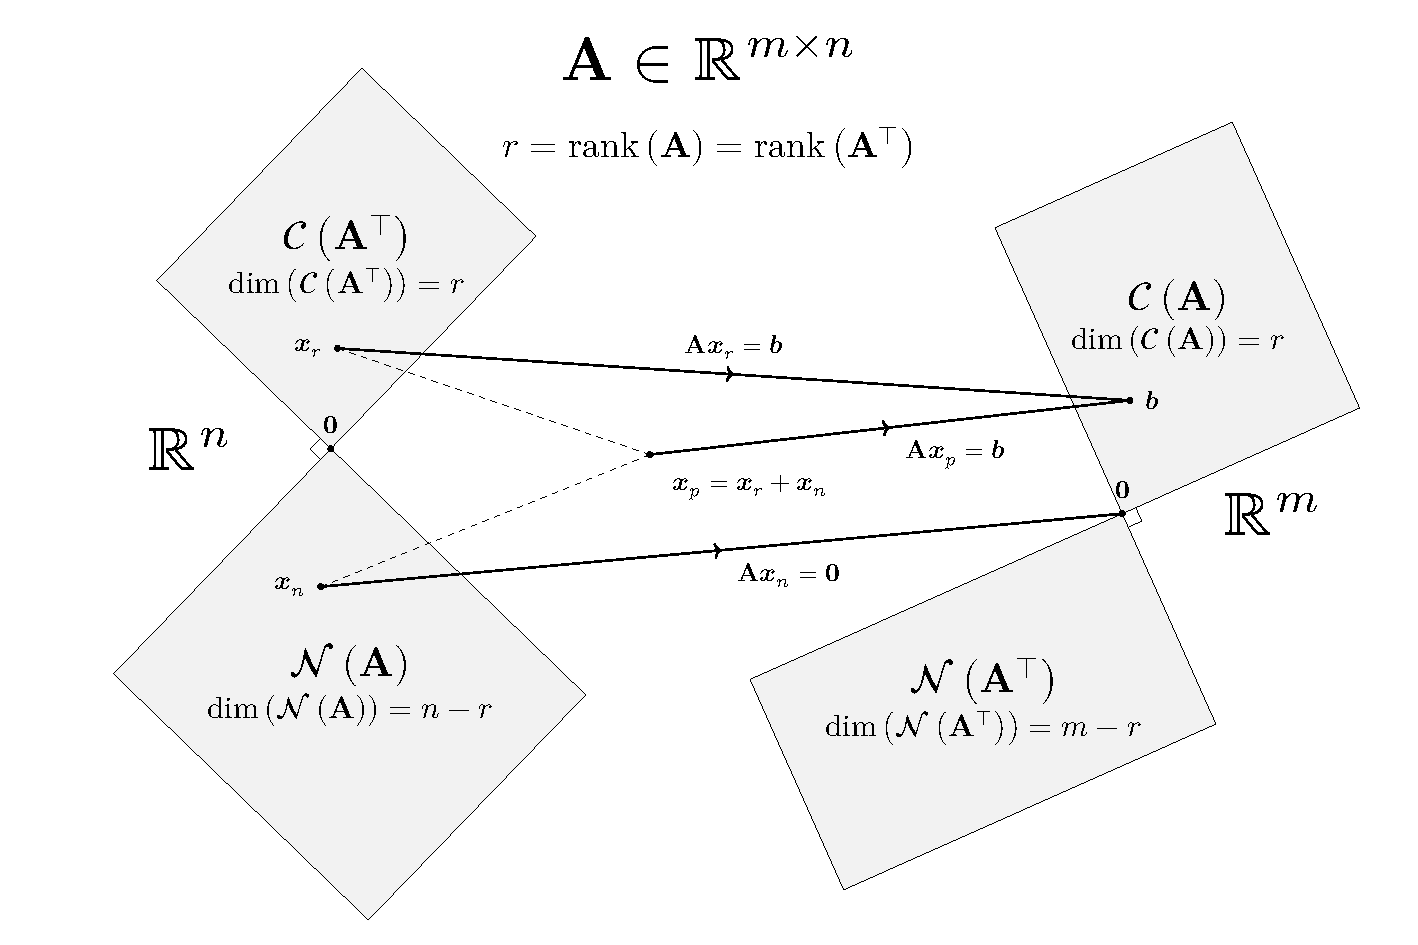
\includegraphics[height = 8cm, keepaspectratio = true]{figures/fundamental_subspaces.pdf}
    \caption{The four fundamental subspaces.} % \label{}
\end{figure}
\subsubsection{Dimensions of Subspaces}
For the matrix \(\symbf{A} \in \R^{m \times n}\):
\begin{definition}[Rank]
    The dimension of the row space is called the \textbf{rank} of a matrix.
    \begin{equation*}
        \vrank{\left( \symbf{A} \right)} = \dim{\left( \rowspace{A} \right)} = r
    \end{equation*}
    To determine the rank, we can count the number of basic variables in \(\symbf{R}\).

    Note that the \(\vrank{\left( \symbf{A} \right)} = \vrank{\left( \symbf{A}^\top \right)}\).
\end{definition}
\begin{definition}[Nullity]
    The dimension of the null space is called the \textbf{nullity} of the matrix.
    \begin{equation*}
        \vnull{\left( \symbf{A} \right)} = \dim{\left( \nullspace{A} \right)}
    \end{equation*}
\end{definition}
\begin{definition}[Left nullity]
    The dimension of the left null space is called the \textbf{left nullity} of the matrix.
    \begin{equation*}
        \vnull{\left( \symbf{A}^\top \right)} = \dim{\left( \leftnullspace{A} \right)}
    \end{equation*}
\end{definition}
\begin{theorem}[Rank-nullity theorem]
    The dimension of the domain of \(\symbf{A}\), \(\R^n\), is given by
    the sum of the dimensions of the row space and null space of \(\symbf{A}\).
    \begin{align*}
        \dim{\left( \rowspace{A} \right)} + \dim{\left( \nullspace{A} \right)} & = \dim{\left( \R^n \right)} \\
        \vrank{\left( \symbf{A} \right)} + \vnull{\left( \symbf{A} \right)}    & = n                         \\
        r + \vnull{\left( \symbf{A} \right)}                                   & = n
    \end{align*}
    Therefore
    \begin{equation*}
        \vnull{\left( \symbf{A} \right)} = n - r
    \end{equation*}
\end{theorem}
\begin{corollary}[Rank-nullity theorem for the transpose]
    The dimension of the codomain of \(\symbf{A}\), \(\R^m\), is given by
    the sum of the dimensions of the column space and left-null space of \(\symbf{A}\).
    \begin{align*}
        \dim{\left( \columnspace{A} \right)} + \dim{\left( \leftnullspace{A} \right)} & = \dim{\left( \R^m \right)} \\
        \vrank{\left( \symbf{A}^\top \right)} + \vnull{\left( \symbf{A}^\top \right)} & = m                         \\
        r + \vnull{\left( \symbf{A}^\top \right)}                                     & = m
    \end{align*}
    Therefore
    \begin{equation*}
        \vnull{\left( \symbf{A}^\top \right)} = m - r
    \end{equation*}
\end{corollary}
\begin{theorem}[Orthogonality of subspaces]
    The row space and null space are orthogonal complements in \(\R^n\).
    \begin{equation*}
        \rowspace{A}^\perp = \nullspace{A}
    \end{equation*}
    Similarly, the column space and left-null space are orthogonal complements in \(\R^m\).
    \begin{equation*}
        \columnspace{A}^\perp = \leftnullspace{A}
    \end{equation*}
\end{theorem}
\subsection{Consistency of a Linear System}
Given a matrix \(\symbf{A} \in \R^{m \times n}\), the linear system \(\symbf{A}\symbfit{x} = \symbfit{b}\),
with any vector \(\symbfit{b}\) can be described as follows:
\begin{enumerate}
    \item Consistent with unique solution:
          \begin{equation*}
              \vrank{\left( \symbf{A} \right)} =
              \vrank{\left( \begin{bmatrix}[c|c]
                      \symbf{A} & \symbfit{b}
                  \end{bmatrix} \right)} = n
          \end{equation*}
    \item Consistent with infinitely many solutions:
          \begin{equation*}
              \vrank{\left( \symbf{A} \right)} =
              \vrank{\left( \begin{bmatrix}[c|c]
                      \symbf{A} & \symbfit{b}
                  \end{bmatrix} \right)}
          \end{equation*}
    \item Inconsistent with no solutions:
          \begin{equation*}
              \vrank{\left( \symbf{A} \right)} \neq
              \vrank{\left( \begin{bmatrix}[c|c]
                      \symbf{A} & \symbfit{b}
                  \end{bmatrix} \right)}
          \end{equation*}
\end{enumerate}
However, if \(\symbfit{b} \in \columnspace{{A}}\), the system must be consistent.
\subsection{General Solution to a Linear System}
Given \(\symbfit{b} \in \columnspace{A}\), the general solution to a system can be expressed as
\begin{equation*}
    \symbfit{x}_g = \symbfit{x}_p + \symbfit{x}_n
\end{equation*}
where \(\symbfit{x}_p\) is a particular solution obtained by backward substitution, and
\(\symbfit{x}_n\) represents the linear combination of all null space basis vectors.
\subsection{Minimum Norm Solution}
In general, the particular solution may contain a linear combination of
null space basis vectors requiring \(\symbfit{x}_p \in \R^n\).

If we consider the solution vector \(\symbfit{x}_r \in \rowspace{A}\), then this vector
will be the minimum norm solution to \(\symbf{A}\symbfit{x} = \symbfit{b}\).
\section{Least Squares}
Given an inconsistent system \(\symbf{A}\symbfit{x} = \symbfit{b}\), we can consider an approximate solution such that we
minimise the norm of the residual:
\begin{equation*}
    \norm{\symbfit{b} - \symbf{A}\symbfit{x}}
\end{equation*}
Therefore we solve the following minimisation problem
\begin{equation*}
    \symbfit{x} = \argmin_{\symbfit{x}^\ast \in \R^n} \norm{\symbfit{b} - \symbf{A}\symbfit{x}}
\end{equation*}
which is known as the \textbf{Least Squares} problem.
\begin{theorem}[Minimum norm solution]
    The solution to the least squares problem is obtained by the vector \(\symbfit{x}\) such
    that \(\symbfit{b} - \symbf{A}\symbfit{x}\) is orthogonal to the column space of \(\symbf{A}\).
\end{theorem}
\subsection{Normal Equations}
Given that \(\symbfit{b} - \symbf{A}\symbfit{x}\) is orthogonal to \(\columnspace{A}\), it must lie in the
left-null space of \(\symbfit{A}\). By orthogonality, we form the following relationship
\begin{equation*}
    \symbf{A}^\top \left( \symbfit{b} - \symbf{A}\symbfit{x} \right) = \symbfit{0}
\end{equation*}
which is equivalent to solving
\begin{equation*}
    \symbf{A}^\top \symbf{A}\symbfit{x} = \symbf{A}^\top \symbfit{b}.
\end{equation*}
This linear equation is known as the \textbf{Normal Equations}, which can be thought of as
a \linebreak generalisation of \(\symbf{A}\symbfit{x} = \symbfit{b}\). But whereas \(\symbf{A}\symbfit{x} = \symbfit{b}\)
can be inconsistent, the normal equations are always consistent.
\subsection{Orthogonal Projection}
By rearranging the normal equations, we can directly compute the solution vector.
\begin{equation*}
    \symbfit{x} = \left( \symbf{A}^\top \symbf{A} \right)^{-1} \symbf{A}^\top \symbfit{b}
\end{equation*}
The projection of \(\symbfit{b}\) onto \(\columnspace{A}\) is therefore
\begin{align*}
    \symbfit{b}_P & = \proj_{\columnspace{A}} \left( \symbfit{b} \right)                                \\
                  & = \symbf{A} \symbfit{x}                                                             \\
                  & = \symbf{A} \left( \symbf{A}^\top \symbf{A} \right)^{-1} \symbf{A}^\top \symbfit{b}
\end{align*}
We can identify the matrix
\begin{equation*}
    \symbf{P} = \symbf{A} \left( \symbf{A}^\top \symbf{A} \right)^{-1} \symbf{A}^\top
\end{equation*}
as the orthogonal projector onto the column space of \(\symbf{A}\), so that it operates on \(\symbfit{b}\):
\begin{equation*}
    \symbf{P} \symbfit{b} = \proj_{\columnspace{A}} \left( \symbfit{b} \right)
\end{equation*}
\begin{definition}[Idempotent]
    A matrix \(\symbf{P}\) is idempotent if it satisfies
    \begin{equation*}
        \symbf{P}^2 = \symbf{P}
    \end{equation*}
\end{definition}
\begin{theorem}
    Given that \(\symbf{P}\symbfit{b}\) produces the projection vector \(\symbfit{b}_P\),
    taking the orthogonal projection of \(\symbfit{b}_P\) again results in the vector \(\symbfit{b}_P\).
    \begin{align*}
        \symbf{P} \symbfit{b}_P        & = \symbfit{b}_P         \\
        \symbf{P}\symbf{P} \symbfit{b} & = \symbf{P} \symbfit{b} \\
        \symbf{P}^2 \symbfit{b}        & = \symbf{P} \symbfit{b}
    \end{align*}
    Therefore orthogonal projectors are idempotent matrices as \(\symbf{P}^2 = \symbf{P}\).
\end{theorem}
\begin{proof}
    If we express the orthogonal projector in its full form, we can verify the result from above
    \begin{align*}
        \symbf{P}^2 & = \symbf{P} \symbf{P}                                                                                                                                           \\
                    & = \symbf{A} \left( \symbf{A}^\top \symbf{A} \right)^{-1} \symbf{A}^\top \symbf{A} \left( \symbf{A}^\top \symbf{A} \right)^{-1} \symbf{A}^\top                   \\
                    & = \symbf{A} \cancel{\left( \symbf{A}^\top \symbf{A} \right)^{-1}} \cancel{\symbf{A}^\top \symbf{A}} \left( \symbf{A}^\top \symbf{A} \right)^{-1} \symbf{A}^\top \\
                    & = \symbf{A} \left( \symbf{A}^\top \symbf{A} \right)^{-1} \symbf{A}^\top                                                                                         \\
                    & = \symbf{P}
    \end{align*}
\end{proof}
\subsection{Dependent Columns}
If \(\symbf{A}\) has dependent columns, then we will obtain an infinite family of Least
Squares solutions. However there will only be one projection vector \(\symbfit{b}_P\).

This arises from \(\nullspace{A} = \mathcal{N}\left(\symbf{A}^\top \symbf{A}\right)\), so that
the solution to the Normal Equations yields
\begin{equation*}
    \symbfit{x} = \symbfit{x}_p + \symbfit{x}_n
\end{equation*}
where \(\symbfit{x}_p\) is the particular Least Squares solution, and \(\symbfit{x}_n\) represents
any linear combination of null space vectors.
\subsection{Orthogonal Projector onto the Column Space}
To obtain a unique solution to the Normal Equations, we can form the matrix \(\symbf{W}\)
such that it has full column rank and it spans the column space of \(\symbf{A}\).
Then the orthogonal projector is given by
\begin{equation*}
    \symbf{P} = \symbf{W} \left( \symbf{W}^\top \symbf{W} \right)^{-1} \symbf{W}^\top
\end{equation*}
\subsection{Orthogonal Projectors onto other Spaces}
Given the orthogonal projector \(\symbf{P} = \proj_V\) onto a subspace \(V\), the
orthogonal projector \(\symbf{Q} = \proj_{V^\perp}\) onto \(V^\perp\) is given by
\begin{equation*}
    \symbf{Q} = \symbf{I} - \symbf{P}
\end{equation*}
This is because the vector \(\symbfit{b}\) can be represented as the
sum of the projections onto \(V\) and \(V^\perp\)
\begin{equation*}
    \symbfit{b} = \symbf{P}\symbfit{b} + \symbf{Q}\symbfit{b}.
\end{equation*}
The dot product of these two vectors is therefore also zero, given that
both projections lie in orthogonal subspaces.
\begin{equation*}
    \left( \symbf{P}\symbfit{b} \right)^\top \symbf{Q}\symbfit{b} = \symbf{0}
\end{equation*}
or
\begin{equation*}
    \symbf{P} \symbf{Q} = \symbf{0}
\end{equation*}
where \(\symbf{0}\) is the zero matrix.
\section{Orthogonal Matrices}
\subsection{Standard Basis Vectors}
The standard basis vectors are constructed by placing a \(1\)
in the \(n\)th row of the \(n\)th basis vector in \(\R^n\).
\begin{equation*}
    \symbfit{e}_1 =
    \begin{bmatrix}
        1      \\
        0      \\
        \vdots \\
        0
    \end{bmatrix}
    ,\: \dots,\: \symbfit{e}_n =
    \begin{bmatrix}
        0      \\
        0      \\
        \vdots \\
        1
    \end{bmatrix}
\end{equation*}
\subsection{Standard Basis}
In \(\R^n\), the standard basis \(S\) consists of the vectors
\begin{equation*}
    S = \left\{ \symbfit{e}_1,\: \dots,\: \symbfit{e}_n \right\}
\end{equation*}
where the coefficients of a column vector implicitly represent the coefficients
of the linear \linebreak combination of basis vectors in \(S\).

For example, the vector \(\symbfit{b}\) in the standard basis
\begin{equation*}
    \symbfit{b} = b_1 \symbfit{e}_1 + \cdots + b_n \symbfit{e}_n
\end{equation*}
can be explicitly represented as a column vector
\begin{equation*}
    \left( \symbfit{b} \right)_S = \begin{bmatrix}
        b_1    \\
        \vdots \\
        b_n
    \end{bmatrix}
\end{equation*}
where \(b_1,\: \dots,\: b_n\) are the entries of \(\left( \symbfit{b} \right)_S\) with respect to the standard basis \(S\).
\subsection{Change of Basis}
To represent the vector \(\symbfit{b}\) in terms of another basis
\(W\), where
\begin{equation*}
    W = \left\{ \symbfit{w}_1,\: \dots,\: \symbfit{w}_n \right\}
\end{equation*}
we must determine the components of each basis vector in \(W\) that
contributes to \(\symbfit{b}\). This is represented by the system:
\begin{align*}
    \symbfit{b} & = c_1 \symbfit{w}_1 + \cdots + c_n \symbfit{w}_n \\
    \symbfit{b} & = \begin{bmatrix}
                        \vertbar      &        & \vertbar      \\
                        \symbfit{w}_1 & \cdots & \symbfit{w}_n \\
                        \vertbar      &        & \vertbar
                    \end{bmatrix} \begin{bmatrix}
                                      c_1    \\
                                      \vdots \\
                                      c_n
                                  \end{bmatrix}         \\
    \symbfit{b} & = \symbf{W} \symbfit{c}
\end{align*}
The component vector \(\symbfit{c}\) is precisely the representation of \(\symbfit{b}\)
with respect to the basis \(W\), so that
\begin{equation*}
    \left( \symbfit{b} \right)_W = \symbfit{c}.
\end{equation*}
\subsection{Orthonormal Basis}
If we consider a basis \(Q\), such that every basis vector is normalised
and orthogonal to every other basis vector, then \(Q\) is an orthonormal basis.
\begin{definition}[Kronecker delta]
    We can summarise such a basis using the Kronecker delta \(\delta_{ij}\),
    which is defined
    \begin{equation*}
        \delta_{ij} = \begin{cases}
            1, & i = j   \\
            0, & i \ne j
        \end{cases}
    \end{equation*}
    so that in an orthonormal basis \(Q\) with basis vectors
    \(\left\{ \symbfit{q}_1,\: \dots,\: \symbfit{q}_n \right\}\)
    \begin{equation*}
        \symbfit{q}_i^\top \symbfit{q}_j = \delta_{ij}
    \end{equation*}
\end{definition}
By using an orthonormal basis, we can determine the coefficients of \(\left( \symbfit{b} \right)_Q\) without
the need to solve a linear system. For example, the \(i\)th coefficient can be determined as
follows
\begin{align*}
    \symbfit{b}                    & = c_1 \symbfit{q}_1 + \cdots + c_n \symbfit{q}_n                                                                                                                                 \\
    \symbfit{q}_i^\top \symbfit{b} & = \symbfit{q}_i^\top \left( c_1 \symbfit{q}_1 + \cdots + c_i \symbfit{q}_i + \cdots + c_n \symbfit{q}_n \right)                                                                  \\
    \symbfit{q}_i^\top \symbfit{b} & = c_1 \cancelto{0}{\symbfit{q}_i^\top \symbfit{q}_1} + \cdots + c_i \cancelto{1}{\symbfit{q}_i^\top \symbfit{q}_i} + \cdots + c_n \cancelto{0}{\symbfit{q}_i^\top \symbfit{q}_n} \\
    \symbfit{q}_i^\top \symbfit{b} & = c_i                                                                                                                                                                            \\
    \symbf{Q}^\top \symbfit{b}     & = \symbfit{c}
\end{align*}
Therefore
\begin{align*}
    \left( \symbfit{b} \right)_Q & = \symbf{Q}^\top \symbfit{b}
\end{align*}
\subsection{Orthogonal Matrices}
To confirm that \(Q = \left\{ \symbfit{q}_1,\: \dots,\: \symbfit{q}_n \right\}\) is an orthonormal basis, we need to confirm that \(\symbfit{q}_i^\top \symbfit{q}_j = \delta_{ij}\) holds for
all basis vectors \(\symbfit{q}_i\).
To do so, we can construct the matrix product \(\symbf{Q}^\top \symbf{Q}\), so that
\begin{align*}
    \symbf{Q}^\top \symbf{Q} & = \begin{bmatrix}
                                     \horzbar & \symbfit{q}_1 & \horzbar \\
                                              & \vdots                   \\
                                     \horzbar & \symbfit{q}_n & \horzbar
                                 \end{bmatrix} \begin{bmatrix}
                                                   \vertbar      &        & \vertbar      \\
                                                   \symbfit{q}_1 & \cdots & \symbfit{q}_n \\
                                                   \vertbar      &        & \vertbar
                                               \end{bmatrix}                         \\
                             & = \begin{bmatrix}
                                     \symbfit{q}_1^\top \symbfit{q}_1 & \cdots & \symbfit{q}_1^\top\symbfit{q}_n  \\
                                     \vdots                           & \ddots & \vdots                           \\
                                     \symbfit{q}_n^\top \symbfit{q}_1 & \cdots & \symbfit{q}_n^\top \symbfit{q}_n
                                 \end{bmatrix} \\
                             & = \begin{bmatrix}
                                     1      & 0      & \cdots & 0      \\
                                     0      & 1      & \ddots & \vdots \\
                                     \vdots & \ddots & \ddots & 0      \\
                                     0      & \cdots & 0      & 1
                                 \end{bmatrix}                                            \\
                             & = \symbf{I}.
\end{align*}
\begin{definition}[Orthogonal Matrices]
    A square matrix \(\symbf{Q}\) is \textit{orthogonal} if it satisfies
    \begin{equation*}
        \symbf{Q}^\top = \symbf{Q}^{-1}
    \end{equation*}
    so that
    \begin{equation*}
        \symbf{Q}^\top \symbf{Q} = \symbf{Q}\symbf{Q}^\top = \symbf{I}.
    \end{equation*}
\end{definition}
\subsection{Projection onto a Vector}
Consider a subspace which consists of one vector \(\symbfit{a}\), the projection of \(\symbfit{b}\)
onto \(\symbfit{a}\) is given by
\begin{align*}
    \proj_{\symbfit{a}} \left( \symbfit{b} \right) = \symbfit{b}_P & = \symbfit{a} \left( \symbfit{a}^\top \symbfit{a} \right)^{-1} \symbfit{a}^\top \symbfit{b} \\
                                                                   & = \frac{\symbfit{a}}{\norm{\symbfit{a}}^2} \symbfit{a} \cdot \symbfit{b}
\end{align*}
If we instead project \(\symbfit{b}\) onto a unit vector \(\symbfit{q}\), then this simplifies to
\begin{equation*}
    \proj_{\symbfit{q}} \left( \symbfit{b} \right) = \symbfit{q} \left( \symbfit{q} \cdot \symbfit{b} \right)
\end{equation*}
\subsection{Gram-Schmidt Process}
To convert an arbitrary basis \(W\)\footnote{Here we use \(W\) to denote the set of vectors that span \(\columnspace{A}\).} to an orthonormal basis \(Q\), we
must develop a process that is generalisable to any basis.

We construct \(Q\) as follows
\begin{align*}
    \symbfit{v}_1 & = \symbfit{w}_1                                                                                                           & \symbfit{q}_1 & = \frac{\symbfit{v}_1}{\norm{\symbfit{v}_1}}  \\
    \symbfit{v}_2 & = \symbfit{w}_2 - \proj_{\symbfit{q}_1} \left( \symbfit{w}_2 \right)                                                      & \symbfit{q}_2 & = \frac{\symbfit{v}_2}{\norm{\symbfit{v}_2}}  \\
    \symbfit{v}_3 & = \symbfit{w}_3 - \proj_{\symbfit{q}_1} \left( \symbfit{w}_3 \right) - \proj_{\symbfit{q}_2} \left( \symbfit{w}_3 \right) & \symbfit{q}_3 & = \frac{\symbfit{v}_3}{\norm{\symbfit{v}_3}}  \\
                  & \vdotswithin{=}                                                                                                           &               & \vdotswithin{=}                               \\
    \symbfit{v}_i & = \symbfit{w}_i - \sum_{j = 1}^{i - 1} \proj_{\symbfit{q}_j} \left( \symbfit{w}_i \right)                                 & \symbfit{q}_i & = \frac{\symbfit{v}_i}{\norm{\symbfit{v}_i}}.
\end{align*}
Using the projection definition for orthogonal vectors, we can simplify this to
\begin{align*}
    \symbfit{v}_1 & = \symbfit{w}_1                                                                                                                                   & \symbfit{q}_1 & = \frac{\symbfit{v}_1}{\norm{\symbfit{v}_1}}  \\
    \symbfit{v}_2 & = \symbfit{w}_2 - \symbfit{q}_1 \left( \symbfit{q}_1 \cdot \symbfit{w}_2 \right)                                                                  & \symbfit{q}_2 & = \frac{\symbfit{v}_2}{\norm{\symbfit{v}_2}}  \\
    \symbfit{v}_3 & = \symbfit{w}_3 - \symbfit{q}_1 \left( \symbfit{q}_1 \cdot \symbfit{w}_3 \right) - \symbfit{q}_2 \left( \symbfit{q}_2 \cdot \symbfit{w}_3 \right) & \symbfit{q}_3 & = \frac{\symbfit{v}_3}{\norm{\symbfit{v}_3}}  \\
                  & \vdotswithin{=}                                                                                                                                   &               & \vdotswithin{=}                               \\
    \symbfit{v}_i & = \symbfit{w}_i - \sum_{j = 1}^{i - 1} \symbfit{q}_j \left( \symbfit{q}_j \cdot \symbfit{w}_i \right)                                             & \symbfit{q}_i & = \frac{\symbfit{v}_i}{\norm{\symbfit{v}_i}}.
\end{align*}
This produces two sets of mutually orthogonal vectors that span the same space as \(W\). Here \(V = \left\{ \symbfit{v}_1,\: \dots,\: \symbfit{v}_n \right\}\) is an orthogonal basis,
and \(Q = \left\{ \symbfit{q}_1,\: \dots,\: \symbfit{q}_n \right\}\) is an orthonormal basis.
\subsection{QR Decomposition}
If we rearrange the steps in the Gram-Schmidt process to solve for \(\symbfit{w}_i\), we get
\begin{align*}
    \symbfit{w}_1 & = \symbfit{q}_1 \norm{\symbfit{v}_1}                                                                                                                                   \\
    \symbfit{w}_2 & = \symbfit{q}_2 \norm{\symbfit{v}_2} + \symbfit{q}_1 \left( \symbfit{q}_1 \cdot \symbfit{w}_2 \right)                                                                  \\
    \symbfit{w}_3 & = \symbfit{q}_3 \norm{\symbfit{v}_3} + \symbfit{q}_1 \left( \symbfit{q}_1 \cdot \symbfit{w}_3 \right) + \symbfit{q}_2 \left( \symbfit{q}_2 \cdot \symbfit{w}_3 \right) \\
                  &                                                                                                                                                                        \\
    \symbfit{w}_i & = \symbfit{q}_i \norm{\symbfit{v}_i} + \sum_{j = 1}^{i - 1} \symbfit{q}_j \left( \symbfit{q}_j \cdot \symbfit{w}_i \right)
\end{align*}
Due to the properties of \(\symbfit{q}_i\), we can also express \(\symbfit{w}_i\) as
\begin{equation*}
    \symbfit{w}_i = \sum_{j = 1}^{i} \symbfit{q}_j \left( \symbfit{q}_j \cdot \symbfit{w}_i \right).
\end{equation*}
And in vector form:
\begin{align*}
    \begin{bmatrix}
        \symbfit{w}_1 & \symbfit{w}_2 & \cdots & \symbfit{w}_n
    \end{bmatrix} & = \begin{bmatrix}
                          \symbfit{q}_1 & \symbfit{q}_2 & \cdots & \symbfit{q}_n
                      \end{bmatrix} \begin{bmatrix}
                                        \norm{\symbfit{v}_1} & \symbfit{q}_1 \cdot \symbfit{w}_2 & \cdots & \symbfit{q}_1 \cdot \symbfit{w}_n       \\[0.2cm]
                                        0                    & \norm{\symbfit{v}_2}              & \ddots & \vdots                                  \\[0.2cm]
                                        \vdots               & \ddots                            & \ddots & \symbfit{q}_{n - 1} \cdot \symbfit{w}_n \\[0.2cm]
                                        0                    & \cdots                            & 0      & \norm{\symbfit{v}_n}
                                    \end{bmatrix} \\
    \symbf{W}                                               & = \symbf{Q} \symbf{R}
\end{align*}
\subsection{Least Squares using QR Decomposition}
Consider \(\symbfit{u} \notin \columnspace{A}\), by using the QR decomposition of \(\symbf{A}\), we have
\begin{align*}
    \symbf{A} \symbfit{c}                          & = \symbfit{u}                 \\
    \left( \symbf{Q} \symbf{R} \right) \symbfit{c} & = \symbfit{u}                 \\
    \symbf{Q}^\top \symbf{Q} \symbf{R} \symbfit{c} & = \symbf{Q}^\top \symbfit{u}  \\
    \symbf{R} \symbfit{c}                          & = \symbf{Q}^\top \symbfit{u}.
\end{align*}
Alternatively, consider the Normal Equations,
\begin{align*}
    \symbf{A}^\top \symbf{A} \symbfit{c}                                                   & = \symbf{A}^\top \symbfit{u}                                                   \\
    \left( \symbf{Q} \symbf{R} \right)^\top \left( \symbf{Q} \symbf{R} \right) \symbfit{c} & = \left( \symbf{Q} \symbf{R} \right)^\top \symbfit{u}                          \\
    \symbf{R}^\top \symbf{Q}^\top \symbf{Q} \symbf{R} \symbfit{c}                          & = \symbf{R}^\top \symbf{Q}^\top \symbfit{u}                                    \\
    \symbf{R}^\top \symbf{R} \symbfit{c}                                                   & = \symbf{R}^\top \symbf{Q}^\top \symbfit{u}                                    \\
    \left( \symbf{R}^\top \right)^{-1} \symbf{R}^\top \symbf{R} \symbfit{c}                & = \left( \symbf{R}^\top \right)^{-1} \symbf{R}^\top \symbf{Q}^\top \symbfit{u} \\
    \symbf{R} \symbfit{c}                                                                  & = \symbf{Q}^\top \symbfit{u}
\end{align*}
Therefore by using the QR decomposition of \(\symbf{A}\) we can find the Least Squares solution \(\symbfit{c}^\ast\), using backward-substitution.
\section{Eigenvalues and Eigenvectors}
\subsection{Linear Operators}
Consider the linear transformation \(T\) that maps any vector
\(\symbfit{v}\in V\) to \(V\). \(T\) is referred to as a linear operator from \(V\) to \(V\):
\begin{equation*}
    T:V \to V.
\end{equation*}
\subsection{The Eigenvalue Problem}
Given the linear transformation
\begin{equation*}
    \symbfit{v} \mapsto \symbf{A} \symbfit{v}
\end{equation*}
for \(\symbf{A}\in\R^{n \times n}\), let \(\symbfit{v}\) be an eigenvector of \(\symbf{A}\)
and \(\lambda\) its associated eigenvalue so that the following relationship is
satisfied,
\begin{equation*}
    \symbf{A}\symbfit{v} = \lambda \symbfit{v}.
\end{equation*}
These eigenvalue and eigenvector pairs form eigenpairs of \(\symbf{A}\).
\subsection{Calculating Eigenvalues}
By rearranging the eigenvalue problem we have,
\begin{align*}
    \symbf{A}\symbfit{v}                                    & = \lambda \symbfit{v}           \\
    \symbf{A}\symbfit{v}                                    & = \lambda \symbf{I} \symbfit{v} \\
    \lambda \symbf{I} \symbfit{v} - \symbf{A}\symbfit{v}    & = \symbf{0}                     \\
    \left( \lambda \symbf{I} - \symbf{A} \right)\symbfit{v} & = \symbf{0}.
\end{align*}
For this homogeneous linear system to have non-trivial solutions, the rank of the coefficient matrix \(\lambda \symbf{I} - \symbf{A}\)
must be less than \(n\). This requires the matrix to be singular so that its determinant is equal to \(0\):
\begin{equation*}
    \det{\left( \lambda \symbf{I} - \symbf{A} \right)} = 0.
\end{equation*}
\begin{definition}[Characteristic polynomial]
    Let \(P\left( \lambda \right)\) denote the resulting polynomial of degree \(n\):
    \begin{equation*}
        P\left( \lambda \right) = \det{\left( \lambda \symbf{I} - \symbf{A} \right)}.
    \end{equation*}
\end{definition}
We use \(\lambda \symbf{I} - \symbf{A}\) rather than \(\symbf{A} - \lambda \symbf{I}\) to ensure that the polynomial is monic,
i.e.\ the leading coefficient is equal to \(1\).
\subsection{Calculating Eigenvectors}
To calculate the eigenvector \(\symbfit{v}_i\) associated with the eigenvalue \(\lambda_i\), we must find the null space
of \(\lambda_i \symbf{I} - \symbf{A}\). As this yields a basis for the null space, any scalar multiple of an eigenvalue also
satisfies the eigenvalue problem.
\begin{definition}[Eigenspace]
    The null space of \(\lambda_i \symbf{I} - \symbf{A}\) is called the eigenspace associated with \(\lambda_i\).
\end{definition}
\subsection{Eigen Decomposition}
The equations formed by all eigenpairs of the matrix \(\symbf{A}\) can be expressed as
\begin{equation*}
    \symbf{A} \symbf{V} = \symbf{V} \symbf{D}
\end{equation*}
which gives us the eigen decomposition or diagonalisation of \(\symbf{A}\),
\begin{equation*}
    \symbf{A} = \symbf{V} \symbf{D} \symbf{V}^{-1}.
\end{equation*}
Here \(\symbf{V}\) is a matrix comprised of the eigenvectors \(\symbfit{v}_i\) as its columns, and \(\symbf{D}\) is a
diagonal matrix of the eigenvalues \(\lambda_i\). Mathematically,
\begin{align*}
    \symbf{V} & = \begin{bmatrix}
                      \symbfit{v}_1 & \cdots & \symbfit{v}_n
                  \end{bmatrix}
              & \symbf{D}                               & = \diag{\left( \lambda_1,\: \dots,\: \lambda_n \right)}
\end{align*}
\begin{definition}[Algebraic multiplicity]
    The algebraic multiplicity \(\mu_{\symbf{A}}\left( \lambda_i \right)\)
    of an eigenvalue \(\lambda_i\) is
    the multiplicity of \(\lambda_i\) in the characteristic polynomial
    (i.e.,\ how many times it is repeated).

    For \(d \leq n\) distinct eigenvalues,
    \begin{equation*}
        P\left( \lambda \right) = 0 = \left( \lambda - \lambda_1 \right)^{\mu_{\symbf{A}}\left( \lambda_1 \right)} \left( \lambda - \lambda_2 \right)^{\mu_{\symbf{A}}\left( \lambda_2 \right)} \cdots \left( \lambda - \lambda_d \right)^{\mu_{\symbf{A}}\left( \lambda_d \right)}.
    \end{equation*}
    This requires
    \begin{gather*}
        1 \leq \mu_{\symbf{A}}\left( \lambda_i \right) \leq n         \\
        \mu_{\symbf{A}} = \sum_{i = 1}^d \mu_{\symbf{A}} \left( \lambda_i \right) = n
    \end{gather*}
\end{definition}
\begin{definition}[Geometric multiplicity]
    The dimension of the eigenspace associated with \(\lambda_i\) is referred to as the
    geometric multiplicity of \(\lambda_i\), denoted \(\gamma_{\symbf{A}}\left( \lambda_i \right)\).

    As the eigenspace is by definition the
    null space of \(\lambda_i \symbf{I} - \symbf{A}\),
    \begin{equation*}
        \gamma_{\symbf{A}} \left( \lambda_i \right) = \nullity{\left( \lambda_i \symbf{I} - \symbf{A} \right)}.
    \end{equation*}
    Given \(d \leq n\) distinct eigenvalues,
    \begin{gather*}
        1 \leq \gamma_{\symbf{A}}\left( \lambda_i \right) \leq \mu_{\symbf{A}}\left( \lambda_i \right) \leq n \\
        \gamma_{\symbf{A}} = \sum_{i = 1}^d \gamma_{\symbf{A}} \left( \lambda_i \right)
    \end{gather*}
    so that
    \begin{equation*}
        d \leq \gamma_{\symbf{A}} \leq n.
    \end{equation*}
\end{definition}
\begin{theorem}[Eigenvectors of distinct eigenvalues]
    Eigenvectors corresponding to distinct eigenvalues are linearly dependent.
\end{theorem}
\begin{definition}[Defective matrix]
    A defective matrix is a matrix that does not have a complete basis of eigenvectors and is therefore not diagonalisable.
    In particular, there exists at least one eigenvalue \(\lambda_k\),
    where \(\gamma_{\symbf{A}}\left( \lambda_k \right) < \mu_{\symbf{A}}\left( \lambda_k \right)\)
\end{definition}
\subsection{Matrix Similarity}
\begin{definition}[Similar matrices]
    Two \(n \times n\) matrices \(\symbf{A}\) and \(\symbf{B}\) are similar,
    if there exists an invertible \(n \times n\) matrix \(\symbf{P}\) such that
    \begin{equation*}
        \symbf{B} = \symbf{P}^{-1} \symbf{A} \symbf{P}.
    \end{equation*}
\end{definition}
\begin{theorem}[Characteristic polynomial of similar matrices]
    Two similar matrices \(\symbf{A}\) and \(\symbf{B}\) have the
    same characteristic polynomial \(P\left( \lambda \right)\) so that they share their ranks,
    determinants, trace, and eigenvalues (including their algebraic and geometric multiplicities).
\end{theorem}
\begin{proof}
    The eigenvalues of \(\symbf{B}\) can be determined using the characteristic polynomial:
    \begin{align*}
        P_{\symbf{B}}\left( \lambda \right) & = \det{\left( \lambda \symbf{I} - \symbf{B} \right)}                                                                    \\
                                            & = \det{\left( \lambda \symbf{I} - \symbf{P}^{-1} \symbf{A} \symbf{P} \right)}                                           \\
                                            & = \det{\left( \lambda \symbf{P}^{-1} \symbf{I} \symbf{P} - \symbf{P}^{-1} \symbf{A} \symbf{P} \right)}                  \\
                                            & = \det{\left( \symbf{P}^{-1} \left( \lambda \symbf{I} - \symbf{A} \right) \symbf{P} \right)}                            \\
                                            & = \det{\left( \symbf{P}^{-1} \right)} \det{\left( \lambda \symbf{I} - \symbf{A} \right)} \det{\left( \symbf{P} \right)} \\
                                            & = \det{\left( \symbf{P}^{-1} \symbf{P} \right)} \det{\left( \lambda \symbf{I} - \symbf{A} \right)}                      \\
                                            & = \det{\left( \symbf{I} \right)} \det{\left( \lambda \symbf{I} - \symbf{A} \right)}                                     \\
                                            & = \det{\left( \lambda \symbf{I} - \symbf{A} \right)}                                                                    \\
                                            & = P_{\symbf{A}}\left( \lambda \right)
    \end{align*}
\end{proof}
\subsection{Constructing a Similar Matrix}
Given a diagonalisable matrix \(\symbf{A} = \symbf{V}\symbf{D}\symbf{V}^{-1}\), we can construct the matrix \(\symbf{B}\) with arbitrary eigenvectors
\(\symbf{W}\), so that
\begin{align*}
    \symbf{B} = \symbf{W} \symbf{D} \symbf{W}^{-1}.
\end{align*}
Using \(\symbf{D} = \symbf{V}^{-1} \symbf{A} \symbf{V}\),
\begin{align*}
    \symbf{B} & = \symbf{W} \symbf{D} \symbf{W}^{-1}                                               \\
              & = \symbf{W} \left( \symbf{V}^{-1} \symbf{A} \symbf{V} \right) \symbf{W}^{-1}       \\
              & = \left( \symbf{V} \symbf{W}^{-1} \right)^{-1} \symbf{A} \symbf{V} \symbf{W}^{-1}.
\end{align*}
Let \(\symbf{P} = \symbf{V} \symbf{W}^{-1}\), so that
\begin{equation*}
    \symbf{B} = \symbf{P}^{-1} \symbf{A} \symbf{P}.
\end{equation*}
This result shows us that \(\symbf{A}\) and \(\symbf{B}\) are similar matrices.
\subsection{Symmetric Matrices}
Consider the symmetric matrix \(\symbf{A}\in\R^{n \times n}\) where \(\symbf{A}^\top = \symbf{A}\).
Then:
\begin{enumerate}
    \item \(\symbf{A}\) is always diagonalisable.
    \item The eigenvalues and eigenvectors of symmetric matrices are always real.
    \item The eigenspaces of a symmetric matrix are orthogonal for \(\lambda_i \neq \lambda_j\).
\end{enumerate}
\subsection{Orthogonal Matrices}
By applying the Gram-Schmidt process to the eigenvectors of a symmetric matrix, we obtain the decomposition
\begin{equation*}
    \symbf{A} = \symbf{Q} \symbf{D} \symbf{Q}^\top
\end{equation*}
where \(\symbf{Q}\) is a diagonal matrix that satisfies \(\symbf{Q}^{-1} = \symbf{Q}^\top\).
\subsection{Definite Matrices}
Symmetric matrices are also known as definite matrices, and can be classified into four categories.
\begin{enumerate}
    \item Positive definite matrices: All eigenvalues are positive.
    \item Positive semidefinite matrices: All eigenvalues are nonnegative.
    \item Negative definite matrices: All eigenvalues are nonpositive.
    \item Negative semidefinite matrices: All eigenvalues are negative.
\end{enumerate}
\subsection{Eigenbases}
When \(\symbf{A}\) has \(n\) linearly independent eigenvectors, the columns of \(\symbf{V}\) represent the eigenbasis of \(\symbf{A}\).

Let the basis \(V\) be the columns of \(\symbf{V}\) so that for the linear system \(\symbf{A}\symbfit{x} = \symbfit{b}\),
\(\left[ \symbfit{x} \right]_V = \symbfit{c}\) and \(\left[ \symbfit{b} \right]_V = \symbfit{k}\),
then
\begin{align*}
    \symbf{A} \symbfit{x}                          & = \symbfit{b}                  \\
    \symbf{A} \symbf{V} \symbfit{c}                & = \symbf{V} \symbfit{k}        \\
    \symbf{V}^{-1} \symbf{A} \symbf{V} \symbfit{c} & = \symbfit{k}                  \\
    \symbf{D} \symbfit{c}                          & = \symbfit{k}                  \\
    \symbf{D} \left( \symbfit{x} \right)_V         & = \left( \symbfit{b} \right)_V
\end{align*}
so that, with respect to the eigenbasis, a linear map from \(\R^n\) to \(\R^n\) is represented by the matrix \(\symbf{D}\).
\subsection{Matrix Functions}
Given a nondefective \(\symbf{A} \in \R^{n \times n}\) with the eigendecomposition \(\symbf{A} = \symbf{V} \symbf{D} \symbf{V}^{-1}\),
we can form the following equalities.
\subsubsection{Powers}
For \(k \in \N\),
\begin{equation*}
    \symbf{A}^k = \symbf{V} \symbf{D}^k \symbf{V}^{-1} = \symbf{V} \diag{\left( \lambda_1^k,\: \ldots,\: \lambda_n^k \right)} \symbf{V}^{-1}.
\end{equation*}
\begin{proof}
    We can prove the above theorem using a recursive construction of \(\symbf{A}^k\).
    \begin{align*}
        \symbf{A}^2 = \symbf{A} \symbf{A}   & = \symbf{V} \symbf{D} \cancel{\symbf{V}^{-1} \symbf{V}} \symbf{D} \symbf{V}^{-1} = \symbf{V} \symbf{D}^2 \symbf{V}^{-1}   \\
        \symbf{A}^3 = \symbf{A}^2 \symbf{A} & = \symbf{V} \symbf{D}^2 \cancel{\symbf{V}^{-1} \symbf{V}} \symbf{D} \symbf{V}^{-1} = \symbf{V} \symbf{D}^3 \symbf{V}^{-1}
    \end{align*}
    so that for a positive integer \(k \in \N\),
    \begin{equation*}
        \symbf{A}^k = \symbf{A}^{k - 1} \symbf{A} = \symbf{V} \symbf{D}^{k - 1} \cancel{\symbf{V}^{-1} \symbf{V}} \symbf{D} \symbf{V}^{-1} = \symbf{V} \symbf{D}^k \symbf{V}^{-1}.
    \end{equation*}
\end{proof}
\subsubsection{Polynomials}
Let \(p\left( t \right) = c_0 + c_1 t + c_2 t^2 + \cdots + c_k t^k\) denote a polynomial of degree \(k\), then the matrix polynomial
\(p\left( \symbf{A} \right)\) can be expressed as
\begin{align*}
    p\left( \symbf{A} \right) & = c_0 \symbf{I} + c_1 \symbf{A} + c_2 \symbf{A}^2 + \cdots + c_k \symbf{A}^k                                                                                                     \\
                              & = c_0 \symbf{V} \symbf{I} \symbf{V}^{-1} + c_1 \symbf{V} \symbf{D} \symbf{V}^{-1} + c_2 \symbf{V} \symbf{D}^2 \symbf{V}^{-1} + \cdots + c_k \symbf{V} \symbf{D}^k \symbf{V}^{-1} \\
                              & = \symbf{V} \left( c_0 \symbf{I} + c_1 \symbf{D} + c_2 \symbf{D}^2 + \cdots + c_k \symbf{D}^k \right) \symbf{V}^{-1}                                                             \\
                              & = \symbf{V} p\left( \symbf{D} \right) \symbf{V}^{-1}                                                                                                                             \\
                              & = \symbf{V} \diag{\left( p\left( \lambda_1 \right),\: \ldots,\: p\left( \lambda_n \right) \right)} \symbf{V}^{-1}.
\end{align*}
\subsection{Analytic Functions}
An analytic function can be represented by its Taylor series expansion, allowing us to operate analytic functions on \(\symbf{A}\).
\begin{align*}
    f\left( \symbf{A} \right) & = \symbf{V} f\left( \symbf{D} \right) \symbf{V}^{-1}                                                               \\
                              & = \symbf{V} \diag{\left( f\left( \lambda_1 \right),\: \ldots,\: f\left( \lambda_n \right) \right)} \symbf{V}^{-1}.
\end{align*}
\begin{theorem}[Cayley-Hamilton theorem]
    The characteristic polynomial of a square matrix \(\symbf{A}\) (that is not necessarily diagonalisable)
    is equal to the zero matrix.
    \begin{equation*}
        P\left( \symbf{A} \right) = \symbfup{0}
    \end{equation*}
\end{theorem}
\section{Singular Value Decomposition}
The singular value decomposition (SVD) of \(\symbf{A} \in \R^{m \times n}\) is given by
\begin{equation*}
    \symbf{A} = \symbf{U} \symbf{\Sigma} \symbf{V}^\top
\end{equation*}
where \(\symbf{U} \in \R^{n \times n}\) is an orthogonal matrix, \(\symbf{\Sigma} \in \R^{m \times n}\)
is a diagonal matrix, and \(\symbf{V} \in  \R^{m \times m}\) is
an orthogonal matrix.
\(\symbf{U}\) is known as the left-singular matrix and \(\symbf{V}\) is the right-singular matrix,
corresponding to how these matrices are multiplied to \(\symbf{\Sigma}\).

\(\symbf{\Sigma}\) consists of the \textbf{singular values} \(\sigma_i\) of \(\symbf{A}\), which can be determined
using the following process:
\begin{align*}
    \symbf{A}^\top \symbf{A} & = \left( \symbf{U} \symbf{\Sigma} \symbf{V}^\top \right)^\top \left( \symbf{U} \symbf{\Sigma} \symbf{V}^\top \right) \\
                             & = \symbf{V} \symbf{\Sigma}^\top \symbf{U}^\top \symbf{U} \symbf{\Sigma} \symbf{V}^\top                               \\
                             & = \symbf{V} \symbf{\Sigma}^\top \symbf{\Sigma} \symbf{V}^\top
\end{align*}
similarly,
\begin{align*}
    \symbf{A} \symbf{A}^\top & = \left( \symbf{U} \symbf{\Sigma} \symbf{V}^\top \right) \left( \symbf{U} \symbf{\Sigma} \symbf{V}^\top \right)^\top \\
                             & = \symbf{U} \symbf{\Sigma} \symbf{V}^\top \symbf{V} \symbf{\Sigma}^\top \symbf{U}^\top                               \\
                             & = \symbf{U} \symbf{\Sigma} \symbf{\Sigma}^\top \symbf{U}^\top
\end{align*}
In both instances, we form an orthogonal eigendecomposition where
\(\symbf{\Sigma}^\top \symbf{\Sigma}\) and \(\symbf{\Sigma} \symbf{\Sigma}^\top\) are the eigenvalues of
\(\symbf{A}^\top\symbf{A}\) and \(\symbf{A}\symbf{A}^\top\), respectively.
But because the eigenvalues of \(\symbf{A}^\top\symbf{A}\) and \(\symbf{A}\symbf{A}^\top\)
are equal, \(\symbf{\Sigma}^\top \symbf{\Sigma} = \symbf{\Sigma} \symbf{\Sigma}^\top\).

The singular values are non-negative constants and the entries of \(\symbf{\Sigma}\)
are always non-increasing: \(\sigma_1 \geq \sigma_2 \geq \cdots \geq \sigma_r > 0\)
where \(r\) is the rank of \(\symbf{A}\).
\subsection{Orthonormal Bases for the Fundamental Subspaces}
For \(\symbf{A}\in\R^{m \times n}\) with \(\vrank{\left( \symbf{A} \right)} = r \leq n\):
\begin{equation*}
    \symbf{A} \symbf{V} = \symbf{U} \symbf{\Sigma}
\end{equation*}
with
\begin{align*}
    \symbf{A} \symbf{V}      & = \begin{bmatrix}
                                     \vertbar      &        & \vertbar      & \vertbar          &        & \vertbar      \\
                                     \symbfit{a}_1 & \cdots & \symbfit{a}_r & \symbfit{a}_{r+1} & \cdots & \symbfit{a}_n \\
                                     \vertbar      &        & \vertbar      & \vertbar          &        & \vertbar
                                 \end{bmatrix} \begin{bmatrix}
                                                   \vertbar      &        & \vertbar      & \vertbar          &        & \vertbar      \\
                                                   \symbfit{v}_1 & \cdots & \symbfit{v}_r & \symbfit{v}_{r+1} & \cdots & \symbfit{v}_n \\
                                                   \vertbar      &        & \vertbar      & \vertbar          &        & \vertbar
                                               \end{bmatrix} \\
    \symbf{U} \symbf{\Sigma} & = \begin{bmatrix}
                                     \vertbar      &        & \vertbar      & \vertbar          &        & \vertbar      \\
                                     \symbfit{u}_1 & \cdots & \symbfit{u}_r & \symbfit{u}_{r+1} & \cdots & \symbfit{u}_m \\
                                     \vertbar      &        & \vertbar      & \vertbar          &        & \vertbar
                                 \end{bmatrix} \begin{bmatrix}
                                                   \sigma_1 &        &          &   &        &   \\
                                                            & \ddots &          &   &        &   \\
                                                            &        & \sigma_r &   &        &   \\
                                                            &        &          & 0 &        &   \\
                                                            &        &          &   & \ddots &   \\
                                                            &        &          &   &        & 0 \\
                                                            &        &          &   &        &   \\
                                                            &        &          &   &        &   \\
                                                            &        &          &   &        &
                                               \end{bmatrix}
    \setlength{\arraycolsep}{0pt} % Avoid any column space in arrays that follow
    \begin{array}{ l }
        \left.\kern-\nulldelimiterspace
        \vphantom{\begin{array}{ c }
                          0 \\ % Second row
                          0 \\ % Third row
                          0     % Fourth/last row
                      \end{array}}
        \right\}\text{\(r\) rows}     \\
        \left.\kern-\nulldelimiterspace
        \vphantom{\begin{array}{ c }
                          0 \\ % Second row
                          0 \\ % Third row
                          0     % Fourth/last row
                      \end{array}}
        \right\}\text{\(n - r\) rows} \\
        \left.\kern-\nulldelimiterspace
        \vphantom{\begin{array}{ c }
                          0 \\ % Second row
                          0 \\ % Third row
                          0     % Fourth/last row
                      \end{array}}
        \right\}\text{\(m - n\) rows}
    \end{array}
\end{align*}
where we have \(r\) singular values because \(\vrank{\symbf{A}} = \vrank{\symbf{A}^\top \symbf{A}}\).
If we express each equation separately, then
\begin{align*}
    \symbf{A} \symbfit{v}_1       & = \sigma_1 \symbfit{u}_1 \\
                                  & \vdotswithin{=}          \\
    \symbf{A} \symbfit{v}_r       & = \sigma_2 \symbfit{u}_r \\
    \symbf{A} \symbfit{v}_{r + 1} & = \symbfup{0}            \\
                                  & \vdotswithin{=}          \\
    \symbf{A} \symbfit{v}_{n}     & = \symbfup{0}
\end{align*}
which shows us that \(\left\{\symbfit{v}_{r+1},\: \dots,\: \symbfit{v}_{n}\right\}\) forms a basis for the null space of \(\symbf{A}\),
requiring the remaining columns of \(\symbf{V}\) to form a basis for the row space of \(\symbf{A}\).

This means that \(\left\{\symbfit{u}_{1},\: \dots,\: \symbfit{u}_{r}\right\}\) also forms a basis for the column space of \(\symbf{A}\),
and hence, the remaining columns of \(\symbf{U}\) form a basis for the left-null space of \(\symbf{A}\).

To summarise:
\begin{align*}
    \rowspace{A}  & = \vspan{\left( \left\{ \symbfit{v}_{i \leq r} \right\} \right)}     & \columnspace{A}   & = \vspan{\left( \left\{ \symbfit{u}_{i \leq r} \right\} \right)}     \\
    \nullspace{A} & = \vspan{\left( \left\{ \symbfit{v}_{r < i \leq n} \right\} \right)} & \leftnullspace{A} & = \vspan{\left( \left\{ \symbfit{u}_{r < i \leq m} \right\} \right)}
\end{align*}
for \(i \in \N\). Additionally, \(\symbf{V}\) forms an orthonormal basis for \(\R^n\) while
\(\symbf{U}\) forms an orthonormal basis for \(\R^m\).
\subsection{Singular Bases}
Consider the bases \(V\) and \(U\) from the columns of the orthogonal matrices \(\symbf{V}\) and \(\symbf{U}\), respectively.
Let \(\left( \symbfit{x} \right)_V = \symbfit{c}\) and \(\left( \symbfit{b} \right)_U = \symbfit{k}\),
so that the system \(\symbf{A} \symbfit{x} = \symbfit{b}\) becomes
\begin{align*}
    \symbf{A} \symbfit{x}                          & = \symbfit{b}                   \\
    \symbf{A} \symbf{V} \symbfit{c}                & = \symbf{U} \symbfit{k}         \\
    \symbf{U}^\top \symbf{A} \symbf{V} \symbfit{c} & = \symbfit{k}                   \\
    \symbf{\Sigma} \symbfit{c}                     & = \symbfit{k}                   \\
    \symbf{\Sigma} \left( \symbfit{x} \right)_V    & = \left( \symbfit{b} \right)_U.
\end{align*}
Therefore, with respect to the orthogonal bases \(V\) and \(U\), the linear map from \(\R^n\) to \(\R^m\) is represented
by the matrix \(\symbf{\Sigma}\).
\subsection{Reduced SVD}
By ignoring the additional \(m - n\) rows in \(\symbf{\Sigma}\), we can form the reduced SVD which removes the
additional ``0'' rows of \(\symbf{\Sigma}\). This results in \(\symbf{U} \in \R^{m \times n}\) and
\(\symbf{\Sigma} \in \R^{n \times n}\).
\begin{equation*}
    \symbf{U} \symbf{\Sigma} = \begin{bmatrix}
        \vertbar      &        & \vertbar      & \vertbar          &        & \vertbar      \\
        \symbfit{u}_1 & \cdots & \symbfit{u}_r & \symbfit{u}_{r+1} & \cdots & \symbfit{u}_n \\
        \vertbar      &        & \vertbar      & \vertbar          &        & \vertbar
    \end{bmatrix} \begin{bmatrix}
        \sigma_1 &        &          &   &        &   \\
                 & \ddots &          &   &        &   \\
                 &        & \sigma_r &   &        &   \\
                 &        &          & 0 &        &   \\
                 &        &          &   & \ddots &   \\
                 &        &          &   &        & 0
    \end{bmatrix}
    \setlength{\arraycolsep}{0pt}
    \begin{array}{ l }
        \left.\kern-\nulldelimiterspace
        \vphantom{\begin{array}{ c }
                          0 \\
                          0 \\
                          0
                      \end{array}}
        \right\}\text{\(r\) rows} \\
        \left.\kern-\nulldelimiterspace
        \vphantom{\begin{array}{ c }
                          0 \\
                          0 \\
                          0
                      \end{array}}
        \right\}\text{\(n - r\) rows}
    \end{array}
\end{equation*}
The reduced SVD also removes the \(m - n\) left-null space basis vectors \(\left\{ \symbfit{u}_{n < i \leq m} \right\}\) from \(\symbf{U}\).
\subsection{Pseudoinverse}
Using the orthogonal basis vectors obtained through the SVD of \(\symbf{A} \in \R^{m \times n}\), we can show that
\(\symbfit{v}_i \mapsto \sigma_i \symbfit{u}_i\) for all \(i \leq r\). Therefore
\begin{equation*}
    \symbf{A} \symbfit{v}_i = \sigma_i \symbfit{u}_i.
\end{equation*}
If we consider the inverse mapping \(\symbfit{u}_i \mapsto \frac{1}{\sigma_i} \symbfit{v}_i\), then
\begin{equation*}
    \symbf{A}^\dagger \symbfit{u}_i = \frac{1}{\sigma_i} \symbfit{v}_i
\end{equation*}
where \(\symbf{A}^\dagger\) is the pseudoinverse of \(\symbf{A}\). To determine \(\symbf{A}^\dagger\),
the above relationship must hold for all \(i \leq r\). If we multiply the RHS by \(\symbfit{u}^\top_i \symbfit{u}_i\)
\begin{equation*}
    \symbf{A}^\dagger \symbfit{u}_i = \frac{1}{\sigma_i} \symbfit{v}_i \symbfit{u}^\top_i \symbfit{u}_i
\end{equation*}
we can show that \(\symbf{A}^\dagger\) takes the form \(\frac{1}{\sigma_i} \symbfit{v}_i \symbfit{u}^\top_i\).
Using the Kronecker Delta definition of orthonormal vectors, we know that the product of two orthonormal basis vectors is 1
for \(i = j\) and 0 for \(i \neq j\). Therefore by taking the sum of all \(\frac{1}{\sigma_i} \symbfit{v}_i \symbfit{u}^\top_i\),
we have
\begin{align*}
    \symbf{A}^\dagger \symbfit{u}_1 & = \left( \frac{1}{\sigma_1} \symbfit{v}_1 \symbfit{u}^\top_1 + \cdots + \frac{1}{\sigma_r} \symbfit{v}_r \symbfit{u}^\top_r \right) \symbfit{u}_1 = \frac{1}{\sigma_1} \symbfit{v}_1 \cancelto{1}{\symbfit{u}^\top_1 \symbfit{u}_1} + \cdots + \frac{1}{\sigma_r} \symbfit{v}_r \cancelto{0}{\symbfit{u}^\top_r \symbfit{u}_1} = \frac{1}{\sigma_1} \symbfit{v}_1 \\
                                    & \vdotswithin{=}                                                                                                                                                                                                                                                                                                                                                   \\
    \symbf{A}^\dagger \symbfit{u}_r & = \left( \frac{1}{\sigma_1} \symbfit{v}_1 \symbfit{u}^\top_1 + \cdots + \frac{1}{\sigma_r} \symbfit{v}_r \symbfit{u}^\top_r \right) \symbfit{u}_r = \frac{1}{\sigma_1} \symbfit{v}_1 \cancelto{0}{\symbfit{u}^\top_1 \symbfit{u}_r} + \cdots + \frac{1}{\sigma_r} \symbfit{v}_r \cancelto{1}{\symbfit{u}^\top_r \symbfit{u}_r} = \frac{1}{\sigma_r} \symbfit{v}_r
\end{align*}
Therefore the pseudoinverse is given by
\begin{equation*}
    \symbf{A}^\dagger = \sum_{i = 1}^r \frac{1}{\sigma_i} \symbfit{v}_i \symbfit{u}^\top_i
\end{equation*}
which is equivalent to
\begin{align*}
    \symbf{A}^\dagger & = \symbf{V} \begin{bmatrix}
                                        \frac{1}{\sigma_1} &        &                    &   &        &   &  &  & \\
                                                           & \ddots &                    &   &        &   &  &  & \\
                                                           &        & \frac{1}{\sigma_r} &   &        &   &  &  & \\
                                                           &        &                    & 0 &        &   &  &  & \\
                                                           &        &                    &   & \ddots &   &  &  & \\
                                                           &        &                    &   &        & 0 &  &  &
                                    \end{bmatrix} \symbf{U}^\top \\
\end{align*}
If we consider the SVD of \(\symbf{\Sigma}\):
\begin{equation*}
    \symbf{\Sigma} = \symbf{U}_\Sigma \symbf{\Sigma}_\Sigma \symbf{V}^\top_\Sigma.
\end{equation*}
we have \(\symbf{U}_\Sigma = \symbf{I}_m\), \(\symbf{\Sigma}_\Sigma = \symbf{\Sigma}\), and \(\symbf{V}_\Sigma = \symbf{I}_n\).
Then the pseudoinverse of this matrix is then
\begin{align*}
    \symbf{\Sigma}^\dagger & = \sum_{i = 1}^r \frac{1}{\sigma_i} \symbfit{v}_{\Sigma,\:i} \symbfit{u}^\top_{\Sigma,\:i} \\
                           & = \begin{bmatrix}
                                   \frac{1}{\sigma_1} &        &                    &   &        &   &  & \\
                                                      & \ddots &                    &   &        &   &  & \\
                                                      &        & \frac{1}{\sigma_r} &   &        &   &  & \\
                                                      &        &                    & 0 &        &   &  & \\
                                                      &        &                    &   & \ddots &   &  & \\
                                                      &        &                    &   &        & 0 &  &
                               \end{bmatrix}
\end{align*}
so that the pseudoinverse of \(\symbf{A}\) can be determined using
\begin{equation*}
    \symbf{A}^\dagger = \symbf{V} \symbf{\Sigma}^\dagger \symbf{U}^\top.
\end{equation*}
Note that the pseudoinverse can also be obtained using the reduced SVD or by using the first \(r\) columns of \(\symbf{U}\) and \(\symbf{V}\) with the \(r \times r\) submatrix of \(\symbf{\Sigma}\).
\subsection{Truncated SVD}
By expanding the SVD of \(\symbf{A}\), we can express it as the sum of rank-1 matrices:
\begin{equation*}
    \symbf{A} = \sum_{i = 1}^n \sigma_i \symbfit{u}_i \symbfit{v}^\top_i.
\end{equation*}
However if \(r < n\), then
\begin{equation*}
    \symbf{A} = \sum_{i = 1}^r \sigma_i \symbfit{u}_i \symbfit{v}^\top_i
\end{equation*}
as \(\sigma_{r < i \leq n} = 0\). As the singular values are ordered from largest to smallest, if we wished to approximate \(\symbf{A}\)
by a matrix of lower rank, we can truncate this sum even further at \(i = \nu\) for \(\nu < r\), to generate a rank-\(\nu\) approximation of \(\symbf{A}\):
\begin{equation*}
    \tilde{\symbf{A}} = \sum_{i = 1}^\nu \sigma_i \symbfit{u}_i \symbfit{v}^\top_i.
\end{equation*}
This allows us to represent the matrix \(\symbf{A}\) using only \(\nu\) singular values and \(2\nu\) singular vectors
(\(\symbfit{u}_i\) and \(\symbfit{v}_i\) for \(i = 1 \ldots \nu\)). This approximate decomposition is known as the truncated SVD\@.
\subsection{Principal Component Analysis}
To summarise, the SVD of \(\symbf{A}\) has three variations in which the dimensions of the decomposition matrices change.
\begin{itemize}
    \item Full SVD\@:
          \begin{equation*}
              \underset{m \times n}{\symbf{A}} = \underset{m \times m}{\symbf{U}} \quad \underset{m \times n}{\symbf{\Sigma}} \quad \underset{n \times n}{\symbf{V}}^\top
          \end{equation*}
    \item Reduced SVD\@:
          \begin{equation*}
              \underset{m \times n}{\symbf{A}} = \underset{m \times n}{\symbf{U}} \quad \underset{n \times n}{\symbf{\Sigma}} \quad \underset{n \times n}{\symbf{V}}^\top
          \end{equation*}
    \item Truncated SVD\@:
          \begin{equation*}
              \underset{m \times n}{\symbf{A}} = \underset{m \times \nu}{\symbf{U}} \quad \underset{\nu \times \nu}{\symbf{\Sigma}} \quad \underset{n \times \nu}{\symbf{V}}^\top
          \end{equation*}
\end{itemize}
Consider the \(i\)th column of \(\symbf{A}\) in the truncated SVD,
\begin{equation*}
    \tilde{\symbf{A}}_{:,\:i} = \symbf{U} \symbf{\Sigma} \symbf{V}_{i,\: :}^\top
\end{equation*}
If we let \(\symbfit{x}_i = \symbf{\Sigma} \symbf{V}_{i,\: :}^\top\), then
\begin{equation*}
    \tilde{\symbf{A}}_{:,\:i} = \symbf{U} \symbfit{x}_i
\end{equation*}
so that \(\symbfit{x}_i \in \R^{\nu}\) is the coordinate vector of \(\tilde{\symbf{A}}_{:,\:i}\) with respect to the basis of left
singular vectors \(\symbf{U}_{:,\: i \leq \nu}\). In statistics or machine learning, the columns of \(\symbf{U}\) are called ``features''
as they are the most important singular vectors used to construct \(\symbf{A}\). The vector \(\symbfit{x}_i\) is then the coordinate
vector of \(\symbf{A}\)'s projection onto the ``feature space''.

In data analysis, this process is referred to as Principal Componenet Analysis (PCA) where the matrix
\(\symbf{A}\) represents a set of observations in which each column contains a particular explanatory variable
that one might be interested in. The model shown above can be used to explain the observations from each
variable in that dataset.
\section{General Vector Spaces}
\subsection{Vector Space Axioms}
A set \(V\) of objects are called ``vectors'' if the following additive and multiplicative axioms
are satisfied \(\forall \symbfit{u}, \symbfit{v}, \symbfit{w} \in V\) and \(\forall k, m \in \R\).
\begin{table}[H]
    \centering
    \begin{tabular}{c c}
        \toprule
        \textbf{Axiom}                      & \textbf{Meaning}                                                                                                    \\
        \midrule
        Closure under vector addition       & \(\symbfit{u} + \symbfit{v} \in V\)                                                                                 \\
        Commutativity of vector addition    & \(\symbfit{u} + \symbfit{v} = \symbfit{v} + \symbfit{u}\)                                                           \\
        Associativity of vector addition    & \(\symbfit{u} + \left( \symbfit{v} + \symbfit{w} \right) = \left( \symbfit{u} + \symbfit{v} \right) + \symbfit{w}\) \\
        Identity element of vector addition & \(\exists \symbfup{0} \in V : \symbfit{u} + \symbfup{0} = \symbfup{0} + \symbfit{u} = \symbfit{u}\)                 \\
        Inverse elements of vector addition & \(\exists \left( -\symbfit{u} \right) \in V : \symbfit{u} + \left( -\symbfit{u} \right) = \symbfup{0}\)             \\
        \bottomrule
    \end{tabular}
    \caption{Additive axioms.} % \label{}
\end{table}
\begin{table}[H]
    \centering
    \begin{tabular}{c c}
        \toprule
        \textbf{Axiom}                                               & \textbf{Meaning}                                                             \\
        \midrule
        Closure under scalar multiplication                          & \(k \symbfit{u} \in V\)                                                      \\
        Distributivity of scalar multiplication with vector addition & \(k \left( \symbfit{u} + \symbfit{v} \right) = k\symbfit{u} + k\symbfit{v}\) \\
        Distributivity of scalar multiplication with scalar addition & \(\left( k + m \right) \symbfit{u} = k\symbfit{u} + m\symbfit{u}\)           \\
        Associativity of scalar multiplication                       & \(k \left( m\symbfit{u} \right) = \left( k m \right) \symbfit{u}\)           \\
        Identity element of scalar multiplication                    & \(1 \symbfit{u} = \symbfit{u}\)                                              \\
        \bottomrule
    \end{tabular}
    \caption{Multiplicative axioms.} % \label{}
\end{table}
If these axioms are satisfied, the objects called ``vectors'' and the operators ``addition'' (\(+\)) and ``scalar multiplication'' (denoted by juxtaposition) form a general vector space \(V\).
It follows that the operations of addition and scalar multiplication need not resemble those in \(\R^n\) to satisfy the 10 axioms described above.
Rather any set with two operations can form a vector space if they satisfy the 10 axioms above.
\subsection{Examples of Vector Spaces}
Aside from the familiar vector space \(\R^n\), we can also consider the following spaces which satisfy the 10 axioms above.
\begin{enumerate}
    \item The set of \(m \times n\) matrices \(\mathscr{M}_{mn}\) with matrix addition and scalar multiplication.
    \item The set of functions \(\mathscr{F}\left( \Omega \right) : \Omega \to \R\) with addition and scalar multiplication defined pointwise.
\end{enumerate}
\end{document}
